
\documentclass[12pt]{article}
\usepackage{times}
\usepackage{setspace}
\setstretch{1.5}
\usepackage{amsmath,amssymb, amsthm}
\usepackage{graphicx}
\usepackage{bm}
\usepackage[hang, flushmargin]{footmisc}
\usepackage[colorlinks=true]{hyperref}
\usepackage[nameinlink]{cleveref}
\usepackage{footnotebackref}
\usepackage{url}
\usepackage{listings}
\usepackage[most]{tcolorbox}
\usepackage{inconsolata}
\usepackage[papersize={8.5in,11in}, margin=1in]{geometry}
\usepackage{float}
\usepackage{caption}
\usepackage{esint}
\usepackage{url}
\usepackage{enumitem}
\usepackage{subfig}
\usepackage{wasysym}
\newcommand{\ilcode}{\texttt}
\usepackage{etoolbox}
\usepackage{physics}
\usepackage{xcolor}
\patchcmd{\thebibliography}{\section*{\refname}}{}{}{}


\makeatletter
\renewcommand{\@seccntformat}[1]{}
\makeatother

\begin{document}



\title{\textbf{CSDS 440: Assignment 4}}

\author{Shaochen (Henry) ZHONG, \ilcode{sxz517} \\ Mingyang TIE, \ilcode{mxt497}}
\date{Due on 09/25/2020, submitted \textcolor{blue}{early} on 09/18/2020}
\maketitle


% % % % % % % % % % % % % % % % % % % % % % % % % % % % % % % % % %
% % % % % % % % % % % % % % % % % % % % % % % % % % % % % % % % % %
% % % % % % % % % % % % % % % % % % % % % % % % % % % % % % % % % %
\section{Problem 15}

Say we have $X$ being a Bernoulli r. v. Let $P(X = 1) = p$ and $P(X = 0) = 1 - p$ we know that its entropy would be:

\begin{align*}
    H(X) &= H_b(p) = -p\log_2(p) - (1-p)\log_2(1-p) \\
    &\Rightarrow H_b'(p) = \log_2(1-p) - \log_2(p)
\end{align*}

Now plot the function.

\begin{figure}[H]
    \centering
    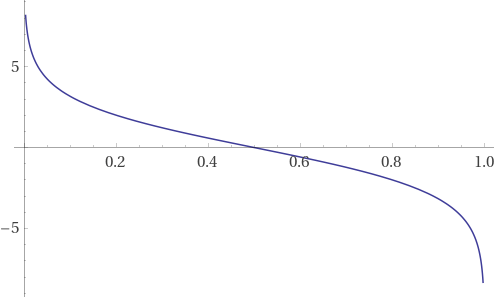
\includegraphics[width=0.4\linewidth]{{fig/fig_p15.png}}
\end{figure}


With the first derivative being a decreasing function, we know the function is concave.



% % % % % % % % % % % % % % % % % % % % % % % % % % % % % % % % % %
% % % % % % % % % % % % % % % % % % % % % % % % % % % % % % % % % %
% % % % % % % % % % % % % % % % % % % % % % % % % % % % % % % % % %
\section{Problem 16}



% % % % % % % % % % % % % % % % % % % % % % % % % % % % % % % % % %
% % % % % % % % % % % % % % % % % % % % % % % % % % % % % % % % % %
% % % % % % % % % % % % % % % % % % % % % % % % % % % % % % % % % %
\section{Problem 17}

% % % % % % % % % % % % % % % % % % % % % % % % % % % % % % % % % %
% % % % % % % % % % % % % % % % % % % % % % % % % % % % % % % % % %
% % % % % % % % % % % % % % % % % % % % % % % % % % % % % % % % % %
\section{Problem 18}


% % % % % % % % % % % % % % % % % % % % % % % % % % % % % % % % % %
% % % % % % % % % % % % % % % % % % % % % % % % % % % % % % % % % %
% % % % % % % % % % % % % % % % % % % % % % % % % % % % % % % % % %
% \section{References}
% \nocite{*}
% \raggedright
% \bibliography{references.bib}
% \bibliographystyle{plain}


\end{document}